% =============================================================================
% Chapter 2: How LLMs Work
% =============================================================================
% This chapter provides the conceptual foundation for understanding hardware
% requirements. Readers will understand WHY transformers need memory before
% Chapter 3 calculates HOW MUCH memory.
% =============================================================================

\chapter{How LLMs Work}
\label{ch:how-llms-work}

\abstract*{Before diving into hardware requirements and VRAM calculations, we need to understand what's actually happening inside these models. This chapter explains transformer architecture from a systems perspective---not the math, but the components and data flow that determine memory usage and performance. By the end, you'll understand why KV cache exists, what the ``billions'' in 7B actually means, and what metrics matter for inference.}

% =============================================================================
\section{From Neural Networks to Transformers}
\label{sec:nn-to-transformers}
% =============================================================================

Neural networks have processed language for decades, but the architectures that preceded transformers had fundamental limitations that made them impractical for today's large language models. Understanding these limitations helps explain why transformers dominate---and why they have the memory characteristics they do.

\subsection{The Sequential Bottleneck}
\label{subsec:sequential-bottleneck}

Before transformers, recurrent neural networks (RNNs) and their variants---LSTMs and GRUs---were the standard for language tasks. These architectures process text one token at a time, maintaining a hidden state that carries information forward through the sequence.

The problem is fundamental: each token's processing depends on the previous token's output. To process ``The cat sat on the mat,'' an RNN must:

\begin{enumerate}
\item Process ``The'' $\rightarrow$ produce hidden state $h_1$
\item Process ``cat'' using $h_1$ $\rightarrow$ produce $h_2$
\item Process ``sat'' using $h_2$ $\rightarrow$ produce $h_3$
\item And so on, strictly sequentially
\end{enumerate}

This sequential dependency creates two critical problems:

\begin{description}
\item[No Parallelization] You cannot process token 5 until tokens 1--4 are complete. Training on long sequences becomes painfully slow because GPUs---designed for parallel computation---sit mostly idle.

\item[Vanishing Context] Information from early tokens must survive through many sequential steps to influence later tokens. In practice, RNNs struggle with long-range dependencies. By token 500, information from token 1 has been diluted through hundreds of transformations.
\end{description}

Researchers tried various fixes: bidirectional RNNs, attention mechanisms bolted onto RNNs, skip connections. These helped, but the fundamental sequential bottleneck remained.

% Diagram: Inference Engine Pipeline
% Shows the flow from request to response through engine components

\begin{figure}[htbp]
\centering
\begin{tikzpicture}[
    node distance=1.2cm and 1.5cm,
    box/.style={rectangle, draw, rounded corners, minimum width=2.2cm, minimum height=1cm, align=center, font=\small},
    arrow/.style={->, thick, >=stealth},
    label/.style={font=\footnotesize\itshape, text=gray}
]

% Top row: Input processing
\node[box, fill=blue!10] (request) {Request\\Handler};
\node[box, fill=green!10, right=of request] (tokenizer) {Tokenizer};
\node[box, fill=orange!10, right=of tokenizer] (forward) {Forward\\Pass};

% Bottom row: Output generation
\node[box, fill=purple!10, below=of forward] (kvcache) {KV Cache\\Manager};
\node[box, fill=red!10, below=of tokenizer] (sampler) {Sampler};
\node[box, fill=blue!10, below=of request] (response) {Response\\Streamer};

% Top row arrows
\draw[arrow] (request) -- (tokenizer);
\draw[arrow] (tokenizer) -- (forward);

% Down and across
\draw[arrow] (forward) -- (kvcache);
\draw[arrow] (kvcache) -- (sampler);
\draw[arrow] (sampler) -- (response);

% Loop back for autoregressive generation (curved path on the right side)
\draw[arrow, dashed, rounded corners=8pt]
    (kvcache.east) -- ++(0.8,0) -- ++(0,1.2) -- ++(-0.8,0) -- (forward.east);
\node[label, anchor=west] at ($(kvcache.east) + (0.9, 0.6)$) {next token};

% Input/Output labels
\node[left=0.5cm of request, font=\small] (input) {``Hello''};
\node[left=0.5cm of response, font=\small] (output) {``Hi!''};
\draw[arrow] (input) -- (request);
\draw[arrow] (response) -- (output);

% Component labels
\node[above=0.15cm of request, label] {API/Queue};
\node[above=0.15cm of tokenizer, label] {Text $\rightarrow$ IDs};
\node[above=0.15cm of forward, label] {GPU Compute};
\node[below=0.15cm of kvcache, label] {Memory Mgmt};
\node[below=0.15cm of sampler, label] {Token Select};
\node[below=0.15cm of response, label] {SSE Stream};

\end{tikzpicture}
\caption{Inference engine pipeline. Requests flow through tokenization and the forward pass (top row), then through KV cache management and sampling (bottom row). The dashed arrow shows the autoregressive loop---each generated token feeds back through the forward pass until generation completes.}
\label{fig:inference-pipeline}
\end{figure}


\subsection{Attention Changes Everything}
\label{subsec:attention-changes}

In 2017, Google researchers published ``Attention Is All You Need''~\cite{vaswani2017attention}, introducing the Transformer architecture. The key insight was radical: remove the sequential processing entirely. Instead of passing information token-by-token through hidden states, let every token directly attend to every other token.

\begin{svgraybox}
\textbf{The Transformer Breakthrough:}

Instead of processing tokens sequentially (1 $\rightarrow$ 2 $\rightarrow$ 3 $\rightarrow$ ...), transformers process all tokens simultaneously. Each token can directly ``look at'' any other token in the sequence, deciding which ones are relevant for its task.
\end{svgraybox}

This architectural change has profound implications:

\begin{description}
\item[Massive Parallelization] During training, all tokens in a sequence can be processed simultaneously. A 4096-token sequence that would take 4096 sequential steps in an RNN can be processed in a single parallel operation. This is why transformers can be trained on billions of tokens---the GPU's parallel processing power is fully utilized.

\item[Direct Long-Range Connections] Token 1 can directly influence token 1000 without information passing through 999 intermediate steps. The model learns which distant tokens are relevant and attends to them directly.

\item[Scalability] The architecture scales with compute. More GPUs means faster training. Larger models with more parameters consistently perform better. This predictable scaling enabled the race to larger models we see today.
\end{description}

% Diagram: Request Flow through Control Plane
% Shows the step-by-step processing of a request

\begin{figure}[htbp]
\centering
\begin{tikzpicture}[
    node distance=0.6cm,
    flowstep/.style={rectangle, draw, rounded corners, minimum width=2.8cm, minimum height=0.7cm, align=center, font=\small},
    arrow/.style={->, thick, >=stealth},
    label/.style={font=\footnotesize\itshape, text=gray}
]

% Left column - Request path
\node[flowstep, fill=blue!15] (req) {1. Request\\Arrives};
\node[flowstep, fill=blue!10, below=of req] (log) {2. Logging\\Middleware};
\node[flowstep, fill=blue!10, below=of log] (metrics1) {3. Metrics\\Middleware};
\node[flowstep, fill=green!15, below=of metrics1] (validate) {4. Validate\\Request};
\node[flowstep, fill=orange!15, below=of validate] (backend) {5. Backend\\Call};

% Right column - Response path
\node[flowstep, fill=orange!15, right=3cm of backend] (process) {6. Process\\Response};
\node[flowstep, fill=purple!15, above=of process] (record) {7. Record\\Metrics};
\node[flowstep, fill=blue!15, above=of record] (resp) {8. Send\\Response};

% Arrows - down the left side
\draw[arrow] (req) -- (log);
\draw[arrow] (log) -- (metrics1);
\draw[arrow] (metrics1) -- (validate);
\draw[arrow] (validate) -- (backend);

% Arrow across to right side
\draw[arrow] (backend) -- node[above, label] {Ollama} (process);

% Arrows - up the right side
\draw[arrow] (process) -- (record);
\draw[arrow] (record) -- (resp);

% Side annotations
\node[label, anchor=east] at ($(req.west) - (0.3, 0)$) {POST /v1/completions};
\node[label, anchor=east] at ($(log.west) - (0.3, 0)$) {assign request\_id};
\node[label, anchor=east] at ($(metrics1.west) - (0.3, 0)$) {start timer};
\node[label, anchor=west] at ($(record.east) + (0.3, 0)$) {histogram, counter};
\node[label, anchor=west] at ($(resp.east) + (0.3, 0)$) {JSON response};

% Time indicator
\draw[<->, gray, dashed] ($(req.east) + (1.2, 0)$) -- ($(backend.east) + (1.2, 0)$);
\node[label, rotate=90] at ($(validate.east) + (1.5, 0)$) {~10ms overhead};

\draw[<->, gray, dashed] ($(backend.east) + (1.2, 0)$) -- ($(process.west) - (0.5, 0)$);
\node[label] at ($(backend.east) + (2.2, 0.3)$) {100ms-60s};
\node[label] at ($(backend.east) + (2.2, -0.1)$) {(inference)};

\end{tikzpicture}
\caption{Request flow through the control plane. Steps 1-4 add ~10ms overhead. Step 5 (inference) dominates latency. The request ID assigned in step 2 appears in all logs, enabling end-to-end tracing.}
\label{fig:request-flow}
\end{figure}


The trade-off is memory. An RNN's memory usage is roughly constant regardless of sequence length---it just maintains a fixed-size hidden state. A transformer's memory grows with sequence length because it must track relationships between all token pairs. For a sequence of $n$ tokens, there are $n^2$ potential attention connections. This quadratic scaling is why context length limits exist and why the KV cache optimization (Section~\ref{sec:kv-cache}) is so important.

\begin{backgroundinformation}{Why ``Attention Is All You Need''?}
The paper's title was provocative. Previous architectures used attention as an add-on to RNNs. The transformer showed that attention alone---without any recurrence---could achieve state-of-the-art results. The ``all you need'' claim has held up remarkably well: seven years later, transformers remain the dominant architecture for language models.
\end{backgroundinformation}

% =============================================================================
\section{Inside a Transformer}
\label{sec:inside-transformer}
% =============================================================================

Now that we understand why transformers replaced RNNs, let's look inside one. We'll focus on the components that matter for inference: what they do, how they use memory, and why they're structured the way they are.

\paragraph{The Two Core Operations}

Every transformer layer performs two fundamental operations:

\begin{enumerate}
\item \textbf{Attention}: Tokens communicate with each other. Each token gathers information from other tokens based on learned relevance weights. This is the ``mixing'' step---information flows between positions.

\item \textbf{Feed-Forward Network (FFN)}: Each token is processed independently. The gathered information is transformed through a neural network. This is the ``thinking'' step---information is processed and refined.
\end{enumerate}

Why both? Consider writing a sentence. Attention is like reading context---``what have I said so far?'' FFN is like reasoning---``given that context, what knowledge applies here?'' Research suggests attention handles \emph{patterns and relationships} while FFN stores \emph{factual knowledge}.

At a high level, each transformer layer computes:
\begin{equation}
\text{Output} = \text{FFN}(\text{Attention}(\text{Input}))
\end{equation}

With residual connections (critical for training deep networks):
\begin{equation}
\begin{aligned}
x' &= x + \text{Attention}(x) \\
\text{Output} &= x' + \text{FFN}(x')
\end{aligned}
\end{equation}

The residual connections let information ``skip'' layers when useful, making deep networks trainable.

\subsection{The High-Level View}
\label{subsec:high-level-view}

The original transformer had two parts: an \emph{encoder} and a \emph{decoder}. Understanding why helps clarify what modern LLMs actually do.

\paragraph{Encoder-Decoder for Translation}

Consider translating ``The cat sat'' to French. This is a \emph{sequence-to-sequence} task: read the entire input, understand it, then produce an output that may have different length and word order (``Le chat s'est assis'').

The encoder reads the full input and builds a rich representation---a ``summary'' of what needs to be translated. The decoder then generates the output word-by-word, consulting that summary. The encoder can look at all words simultaneously (bidirectional attention), while the decoder generates left-to-right.

% Diagram: Traditional vs Paged KV Cache Memory
% Shows memory fragmentation problem and how PagedAttention solves it

\begin{figure}[htbp]
\centering
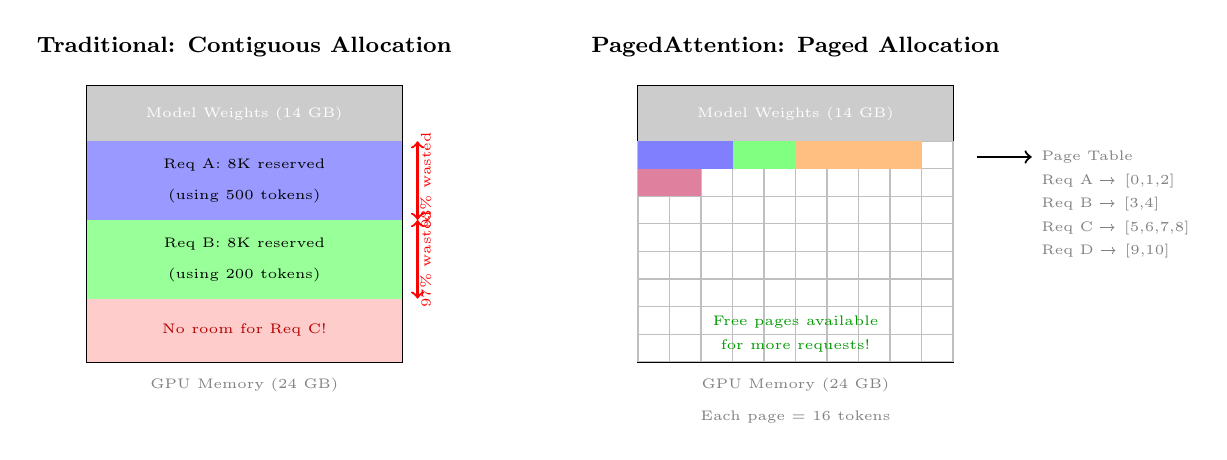
\begin{tikzpicture}[
    node distance=0.2cm,
    memblock/.style={rectangle, draw, minimum height=0.5cm, font=\tiny},
    label/.style={font=\footnotesize},
    timelabel/.style={font=\tiny, text=gray}
]

% === TRADITIONAL ALLOCATION (left) ===
\node[label] at (2, 4) {\textbf{Traditional: Contiguous Allocation}};

% GPU Memory block
\draw[thick] (0, 0) rectangle (4, 3.5);
\node[timelabel] at (2, -0.3) {GPU Memory (24 GB)};

% Model weights (fixed)
\fill[gray!40] (0, 2.8) rectangle (4, 3.5);
\node[font=\tiny, white] at (2, 3.15) {Model Weights (14 GB)};

% KV Cache allocations (pre-allocated for max length)
\fill[blue!40] (0, 1.8) rectangle (4, 2.8);
\node[font=\tiny] at (2, 2.5) {Req A: 8K reserved};
\node[font=\tiny] at (2, 2.1) {(using 500 tokens)};

\fill[green!40] (0, 0.8) rectangle (4, 1.8);
\node[font=\tiny] at (2, 1.5) {Req B: 8K reserved};
\node[font=\tiny] at (2, 1.1) {(using 200 tokens)};

% Wasted space indicator
\fill[red!20] (0, 0) rectangle (4, 0.8);
\node[font=\tiny, red!70!black] at (2, 0.4) {No room for Req C!};

% Fragmentation arrows
\draw[<->, red, thick] (4.2, 1.8) -- (4.2, 2.8);
\node[timelabel, red, rotate=90, anchor=south] at (4.5, 2.3) {93\% wasted};

\draw[<->, red, thick] (4.2, 0.8) -- (4.2, 1.8);
\node[timelabel, red, rotate=90, anchor=south] at (4.5, 1.3) {97\% wasted};

% === PAGED ATTENTION (right) ===
\node[label] at (9, 4) {\textbf{PagedAttention: Paged Allocation}};

% GPU Memory block
\draw[thick] (7, 0) rectangle (11, 3.5);
\node[timelabel] at (9, -0.3) {GPU Memory (24 GB)};

% Model weights (fixed)
\fill[gray!40] (7, 2.8) rectangle (11, 3.5);
\node[font=\tiny, white] at (9, 3.15) {Model Weights (14 GB)};

% Page pool - small fixed-size blocks
\foreach \i in {0,1,2,3,4,5,6,7} {
    \foreach \j in {0,1,2,3,4,5,6,7,8,9} {
        \pgfmathsetmacro{\x}{7 + \j * 0.4}
        \pgfmathsetmacro{\y}{0 + \i * 0.35}
        \draw[gray!50] (\x, \y) rectangle (\x + 0.4, \y + 0.35);
    }
}

% Color used pages
% Req A pages (blue) - scattered
\fill[blue!50] (7, 2.45) rectangle (7.4, 2.8);
\fill[blue!50] (7.4, 2.45) rectangle (7.8, 2.8);
\fill[blue!50] (7.8, 2.45) rectangle (8.2, 2.8);

% Req B pages (green) - scattered
\fill[green!50] (8.2, 2.45) rectangle (8.6, 2.8);
\fill[green!50] (8.6, 2.45) rectangle (9.0, 2.8);

% Req C pages (orange) - can now fit!
\fill[orange!50] (9.0, 2.45) rectangle (9.4, 2.8);
\fill[orange!50] (9.4, 2.45) rectangle (9.8, 2.8);
\fill[orange!50] (9.8, 2.45) rectangle (10.2, 2.8);
\fill[orange!50] (10.2, 2.45) rectangle (10.6, 2.8);

% Req D pages (purple)
\fill[purple!50] (7, 2.1) rectangle (7.4, 2.45);
\fill[purple!50] (7.4, 2.1) rectangle (7.8, 2.45);

% Free pages indicator
\node[timelabel, green!60!black] at (9, 0.5) {Free pages available};
\node[timelabel, green!60!black] at (9, 0.2) {for more requests!};

% Legend
\node[timelabel] at (9, -0.7) {Each page = 16 tokens};

% Page table concept
\draw[->, thick] (11.3, 2.6) -- (12, 2.6);
\node[timelabel, anchor=west] at (12, 2.6) {Page Table};
\node[timelabel, anchor=west, font=\tiny] at (12, 2.3) {Req A → [0,1,2]};
\node[timelabel, anchor=west, font=\tiny] at (12, 2.0) {Req B → [3,4]};
\node[timelabel, anchor=west, font=\tiny] at (12, 1.7) {Req C → [5,6,7,8]};
\node[timelabel, anchor=west, font=\tiny] at (12, 1.4) {Req D → [9,10]};

\end{tikzpicture}
\caption{Traditional vs PagedAttention memory management. Left: Contiguous allocation reserves maximum possible space per request, causing fragmentation and limiting concurrent requests. Right: PagedAttention allocates small fixed-size pages on demand, eliminating fragmentation and enabling 2-4x more concurrent requests.}
\label{fig:paged-attention}
\end{figure}


\paragraph{Why Text Generation Differs}

For translation, you must read everything before producing any output---you can't translate word 1 without knowing word 10 might change the meaning. The encoder-decoder split makes sense.

But for text generation (``write a story about...''), there's no separate ``input'' and ``output.'' You're just continuing a sequence. The prompt and the generated response are the same sequence---the model predicts token $n+1$ from tokens $1$ through $n$, then predicts $n+2$ from $1$ through $n+1$, and so on.

For this task, the encoder is unnecessary overhead. A \emph{decoder-only} model does the job: process the sequence so far, predict the next token. This simpler architecture turns out to be remarkably effective for general-purpose language tasks.

\paragraph{Modern LLM Architecture}

Modern LLMs like GPT, Llama, Mistral, and Qwen are decoder-only transformers. At the highest level:

\begin{enumerate}
\item \textbf{Embedding}: Convert input tokens to vectors (numbers the model can work with)
\item \textbf{Transformer Layers}: Process vectors through many identical layers, each containing attention and feed-forward components
\item \textbf{Output}: Convert final vectors back to token probabilities
\end{enumerate}

% Diagram: Scheduling Considerations
% Shows prefill vs decode phases and scheduling challenges

\begin{figure}[htbp]
\centering
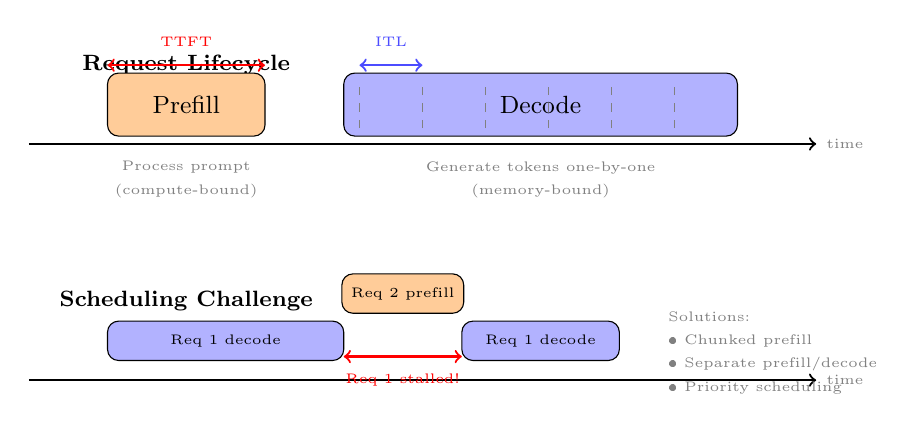
\begin{tikzpicture}[
    node distance=0.5cm,
    phase/.style={rectangle, draw, rounded corners, minimum height=0.8cm, font=\small},
    label/.style={font=\footnotesize},
    timelabel/.style={font=\tiny, text=gray}
]

% === PREFILL VS DECODE ===
\node[label] at (0, 3.5) {\textbf{Request Lifecycle}};

% Single request timeline
\draw[->, thick] (-2, 2.5) -- (8, 2.5) node[right, timelabel] {time};

% Prefill phase
\node[phase, fill=orange!40, minimum width=2cm] at (0, 3) {Prefill};
\node[timelabel] at (0, 2.2) {Process prompt};
\node[timelabel] at (0, 1.9) {(compute-bound)};

% Decode phase
\node[phase, fill=blue!30, minimum width=5cm] at (4.5, 3) {Decode};
\node[timelabel] at (4.5, 2.2) {Generate tokens one-by-one};
\node[timelabel] at (4.5, 1.9) {(memory-bound)};

% TTFT marker
\draw[<->, red, thick] (-1, 3.5) -- (1, 3.5);
\node[timelabel, red] at (0, 3.8) {TTFT};

% ITL markers
\foreach \x in {2.2, 3.0, 3.8, 4.6, 5.4, 6.2} {
    \draw[gray, dashed] (\x, 2.7) -- (\x, 3.3);
}
\draw[<->, blue!70, thick] (2.2, 3.5) -- (3.0, 3.5);
\node[timelabel, blue!70] at (2.6, 3.8) {ITL};

% === SCHEDULING CHALLENGE ===
\node[label] at (0, 0.5) {\textbf{Scheduling Challenge}};

% Multiple requests with prefill interference
\draw[->, thick] (-2, -0.5) -- (8, -0.5) node[right, timelabel] {time};

% Request 1 - already decoding
\node[phase, fill=blue!30, minimum width=3cm, minimum height=0.5cm] at (0.5, 0) {\tiny Req 1 decode};

% Request 2 - prefill arrives, blocks decode
\node[phase, fill=orange!40, minimum width=1.5cm, minimum height=0.5cm] at (2.75, 0.6) {\tiny Req 2 prefill};

% Request 1 continues but delayed
\node[phase, fill=blue!30, minimum width=2cm, minimum height=0.5cm] at (4.5, 0) {\tiny Req 1 decode};

% Stall indicator
\draw[<->, red, thick] (2, -0.2) -- (3.5, -0.2);
\node[timelabel, red] at (2.75, -0.5) {Req 1 stalled!};

% Solution annotation
\node[timelabel, anchor=west] at (6, 0.3) {Solutions:};
\node[timelabel, anchor=west, font=\tiny] at (6, 0) {• Chunked prefill};
\node[timelabel, anchor=west, font=\tiny] at (6, -0.3) {• Separate prefill/decode};
\node[timelabel, anchor=west, font=\tiny] at (6, -0.6) {• Priority scheduling};

\end{tikzpicture}
\caption{Scheduling in LLM inference. Top: A request has two phases---prefill (processing the prompt, compute-bound) and decode (generating tokens, memory-bound). Time to First Token (TTFT) measures prefill latency; Inter-Token Latency (ITL) measures decode speed. Bottom: When a new prefill arrives, it can stall in-flight decode requests, increasing their latency.}
\label{fig:scheduling}
\end{figure}


Each transformer layer has the same structure, repeated many times. A 7B model might have 32 layers; a 70B model might have 80. More layers generally means more sophisticated reasoning capabilities.

\subsection{Attention: What It Actually Does}
\label{subsec:attention-mechanism}

Attention is the mechanism that lets tokens communicate with each other. Think of it like a conference call where each participant can hear everyone else and decide whose input is relevant to their task.

\paragraph{The Dynamic Programming Intuition}

If you're familiar with dynamic programming, attention has a similar flavor. In DP, you compute solutions to subproblems and reuse them. In attention, each token's representation is computed based on weighted combinations of previous representations.

Think of it as: ``To understand token $i$, look at all tokens $1$ through $i$, figure out which ones are relevant, and combine their information.'' This is similar to a DP recurrence where state $i$ depends on all previous states, with learned weights determining the combination.

The key difference from traditional recurrence: instead of a fixed formula like $f(i) = g(f(i-1), f(i-2))$, attention \emph{learns} which previous positions matter and how much. The weights are computed dynamically based on the content of the tokens, not their positions.

\paragraph{Query, Key, Value}

For each token position, attention computes three things:

\begin{description}
\item[Query (Q)] ``What am I looking for?'' Each token generates a query vector representing what information it needs.

\item[Key (K)] ``What do I contain?'' Each token generates a key vector advertising what information it has.

\item[Value (V)] ``What information should I share?'' Each token generates a value vector containing the actual information to pass along.
\end{description}

The attention mechanism matches queries against keys to determine relevance, then retrieves the corresponding values. It's similar to a database lookup: the query is your search term, keys are the index, and values are the data you retrieve.

\begin{svgraybox}
\textbf{Attention as Database Lookup:}

Imagine you're writing ``The cat sat on the \_\_\_'' and need to predict the next word. The token at the blank position generates a query: ``I need context about what was sat upon.'' Each previous token advertises its key: ``I'm an article,'' ``I'm an animal,'' ``I'm a verb,'' etc. The attention mechanism computes similarity between the query and all keys, finding that ``cat'' and ``sat'' are most relevant. It then retrieves their values to inform the prediction.
\end{svgraybox}

Crucially, in decoder-only models, each token can only attend to previous tokens (and itself). Token 5 can look at tokens 1--5, but not tokens 6 onward. This ``causal masking'' ensures the model can't cheat by looking at future tokens during training.

\paragraph{How Causal Masking Works}

The attention mechanism computes similarity scores between all token pairs, then applies softmax to get weights. To prevent attending to future tokens, we add a \emph{mask} before the softmax:

\begin{equation}
\text{Attention}(Q, K, V) = \text{softmax}\left(\frac{QK^T}{\sqrt{d_k}} + M\right) V
\end{equation}

Where $M$ is a triangular mask matrix:
\[
M = \begin{pmatrix}
0 & -\infty & -\infty & -\infty \\
0 & 0 & -\infty & -\infty \\
0 & 0 & 0 & -\infty \\
0 & 0 & 0 & 0
\end{pmatrix}
\]

The $-\infty$ values become 0 after softmax (since $e^{-\infty} = 0$), effectively zeroing out attention to future positions. Token 1 can only attend to itself; token 2 can attend to tokens 1--2; token $n$ can attend to tokens 1--$n$.

% Diagram: Causal Mask
\begin{figure}[htbp]
\centering
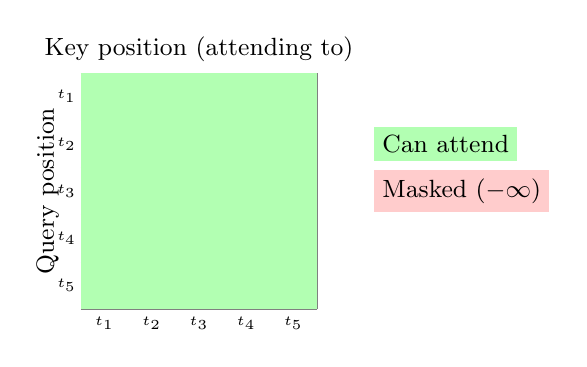
\begin{tikzpicture}[scale=0.6]
% Grid
\draw[step=1cm, gray, very thin] (0,0) grid (5,5);

% Colored cells (lower triangle = can attend)
\foreach \x in {0,...,4} {
    \foreach \y in {0,...,4} {
        \pgfmathtruncatemacro{\sum}{\x + \y}
        \ifnum \y < 5
            \ifnum \x > \y
                \fill[green!30] (\x, 4-\y) rectangle (\x+1, 5-\y);
            \else
                \fill[red!20] (\x, 4-\y) rectangle (\x+1, 5-\y);
            \fi
        \fi
    }
}

% Fix the diagonal and below
\fill[green!30] (0,4) rectangle (1,5);
\fill[green!30] (0,3) rectangle (1,4);
\fill[green!30] (1,3) rectangle (2,4);
\fill[green!30] (0,2) rectangle (1,3);
\fill[green!30] (1,2) rectangle (2,3);
\fill[green!30] (2,2) rectangle (3,3);
\fill[green!30] (0,1) rectangle (1,2);
\fill[green!30] (1,1) rectangle (2,2);
\fill[green!30] (2,1) rectangle (3,2);
\fill[green!30] (3,1) rectangle (4,2);
\fill[green!30] (0,0) rectangle (1,1);
\fill[green!30] (1,0) rectangle (2,1);
\fill[green!30] (2,0) rectangle (3,1);
\fill[green!30] (3,0) rectangle (4,1);
\fill[green!30] (4,0) rectangle (5,1);

% Labels
\node at (2.5, 5.5) {\small Key position (attending to)};
\node[rotate=90] at (-0.7, 2.5) {\small Query position};

% Token labels
\foreach \i in {1,...,5} {
    \node at (\i-0.5, -0.3) {\tiny $t_{\i}$};
    \node at (-0.3, 5.5-\i) {\tiny $t_{\i}$};
}

% Legend
\node[right] at (6, 3.5) {\small \colorbox{green!30}{Can attend}};
\node[right] at (6, 2.5) {\small \colorbox{red!20}{Masked ($-\infty$)}};

\end{tikzpicture}
\caption{Causal attention mask: each token (row) can only attend to itself and earlier tokens (columns).}
\label{fig:causal-mask}
\end{figure}


\subsection{Multi-Head Attention}
\label{subsec:multi-head-attention}

A single attention mechanism learns one way to relate tokens. But language has many types of relationships: grammatical dependencies, semantic similarity, coreference, and more. Multi-head attention runs multiple attention mechanisms in parallel, each learning different relationships.

% Diagram: Multi-Head Attention
\begin{figure}[htbp]
\centering
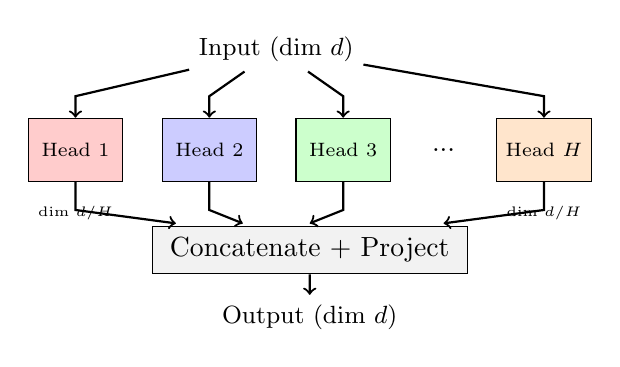
\begin{tikzpicture}[
    scale=0.85,
    head/.style={rectangle, draw, minimum width=1.2cm, minimum height=0.8cm, font=\scriptsize},
    arrow/.style={->, thick}
]
% Input
\node (input) at (0, 3) {\small Input (dim $d$)};

% Split into heads
\node[head, fill=red!20] at (-3, 1.5) (h1) {Head 1};
\node[head, fill=blue!20] at (-1, 1.5) (h2) {Head 2};
\node[head, fill=green!20] at (1, 1.5) (h3) {Head 3};
\node at (2.5, 1.5) {...};
\node[head, fill=orange!20] at (4, 1.5) (hn) {Head $H$};

% Arrows from input
\draw[arrow] (input) -- (-3, 2.3) -- (h1);
\draw[arrow] (input) -- (-1, 2.3) -- (h2);
\draw[arrow] (input) -- (1, 2.3) -- (h3);
\draw[arrow] (input) -- (4, 2.3) -- (hn);

% Concatenate
\node[rectangle, draw, minimum width=4cm, minimum height=0.6cm, fill=gray!10] at (0.5, 0) (concat) {Concatenate + Project};

% Arrows to concat
\draw[arrow] (h1) -- (-3, 0.6) -- (-1.5, 0.4);
\draw[arrow] (h2) -- (-1, 0.6) -- (-0.5, 0.4);
\draw[arrow] (h3) -- (1, 0.6) -- (0.5, 0.4);
\draw[arrow] (hn) -- (4, 0.6) -- (2.5, 0.4);

% Output
\node at (0.5, -1) (output) {\small Output (dim $d$)};
\draw[arrow] (concat) -- (output);

% Annotations
\node[below of=h1, yshift=0.2cm, font=\tiny, align=center] {dim $d/H$};
\node[below of=hn, yshift=0.2cm, font=\tiny, align=center] {dim $d/H$};

\end{tikzpicture}
\caption{Multi-head attention: input is split across $H$ heads, each processing $d/H$ dimensions independently.}
\label{fig:multi-head-attention}
\end{figure}


\paragraph{Why Multiple Heads?}

Consider the sentence: ``The cat that sat on the mat was hungry.'' To predict what comes next, the model needs to track:
\begin{itemize}
\item \textbf{Grammatical structure}: ``was'' agrees with ``cat,'' not ``mat''
\item \textbf{Semantic relationships}: ``hungry'' relates to living things
\item \textbf{Distant dependencies}: ``The cat'' and ``was hungry'' are related despite intervening words
\end{itemize}

A single attention pattern can't capture all these relationships simultaneously. Multiple heads let the model maintain several different ``views'' of token relationships.

\paragraph{The Math (High Level)}

Each head performs its own attention computation on a subset of the dimensions:

\begin{equation}
\text{head}_i = \text{Attention}(Q_i, K_i, V_i) \quad \text{where } Q_i, K_i, V_i \in \mathbb{R}^{n \times d_h}
\end{equation}

All heads are concatenated and projected:

\begin{equation}
\text{MultiHead}(Q, K, V) = \text{Concat}(\text{head}_1, ..., \text{head}_H) W^O
\end{equation}

Where $d_h = d / H$ (head dimension), so the total dimension is preserved.

From a systems perspective, multi-head attention is embarrassingly parallel---all heads compute simultaneously. This is why GPUs excel at transformer inference: the parallel heads map naturally to parallel GPU cores.

\begin{table}[htbp]
\centering
\caption{Attention head configurations in common models.}
\label{tab:attention-heads}
\begin{tabular}{lrrrr}
\toprule
\textbf{Model} & \textbf{Layers} & \textbf{Heads} & \textbf{Head Dim} & \textbf{Model Dim} \\
\midrule
Llama 3.2 7B   & 32 & 32 & 128 & 4096 \\
Mistral 7B    & 32 & 32 & 128 & 4096 \\
Llama 3.1 70B  & 80 & 64 & 128 & 8192 \\
Qwen 2.5 72B   & 80 & 64 & 128 & 8192 \\
\bottomrule
\end{tabular}
\end{table}

Note: $\text{Heads} \times \text{Head Dim} = \text{Model Dim}$. The heads divide the model's representation space, each working on its own subspace.

\subsection{Feed-Forward Networks}
\label{subsec:feed-forward}

After attention lets tokens gather information from each other, each token passes through a feed-forward network (FFN). Unlike attention, the FFN processes each token independently---no communication between positions.

% Diagram: FFN Structure
\begin{figure}[htbp]
\centering
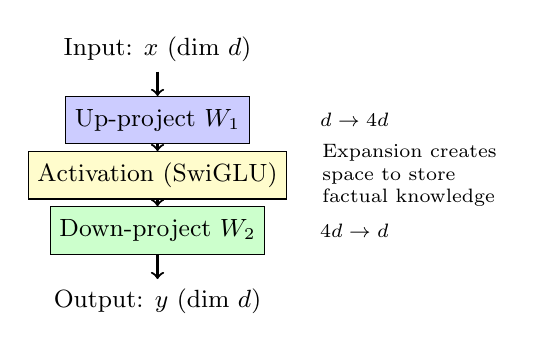
\begin{tikzpicture}[
    node distance=0.7cm,
    block/.style={rectangle, draw, minimum width=2cm, minimum height=0.6cm, font=\small},
    arrow/.style={->, thick}
]
% Input
\node (input) {\small Input: $x$ (dim $d$)};

% Expand
\node[block, fill=blue!20, below of=input, yshift=-0.2cm] (up) {Up-project $W_1$};
\node[right of=up, xshift=1.8cm, font=\scriptsize] {$d \rightarrow 4d$};

% Activation
\node[block, fill=yellow!20, below of=up] (act) {Activation (SwiGLU)};

% Contract
\node[block, fill=green!20, below of=act] (down) {Down-project $W_2$};
\node[right of=down, xshift=1.8cm, font=\scriptsize] {$4d \rightarrow d$};

% Output
\node[below of=down, yshift=-0.2cm] (output) {\small Output: $y$ (dim $d$)};

% Arrows
\draw[arrow] (input) -- (up);
\draw[arrow] (up) -- (act);
\draw[arrow] (act) -- (down);
\draw[arrow] (down) -- (output);

% Annotation
\node[right of=act, xshift=2.5cm, align=left, font=\scriptsize] {Expansion creates\\space to store\\factual knowledge};

\end{tikzpicture}
\caption{Feed-forward network: expand, activate, contract. Most parameters live here.}
\label{fig:ffn-structure}
\end{figure}


\paragraph{Why Expand and Contract?}

The FFN is where much of the model's factual knowledge is stored. Research suggests that attention handles relationships and routing, while FFNs store and recall facts. When a model ``knows'' that Paris is the capital of France, that knowledge likely lives in the FFN weights.

The expansion (typically 4x) creates a larger intermediate space. Think of it as a ``scratchpad'' with more room to represent knowledge. The contraction forces the model to compress back to the original dimension, keeping only what's useful.

\paragraph{The Math}

The classic FFN formula:
\begin{equation}
\text{FFN}(x) = W_2 \cdot \text{activation}(W_1 \cdot x + b_1) + b_2
\end{equation}

Where:
\begin{itemize}
\item $W_1 \in \mathbb{R}^{4d \times d}$ expands from $d$ to $4d$ dimensions
\item $W_2 \in \mathbb{R}^{d \times 4d}$ contracts from $4d$ back to $d$
\item activation is typically ReLU, GELU, or SwiGLU
\end{itemize}

Modern models use \textbf{SwiGLU}, which has a gating mechanism:
\begin{equation}
\text{SwiGLU}(x) = (\text{Swish}(W_1 x) \otimes W_3 x) W_2
\end{equation}

This adds a third weight matrix but improves performance.

\paragraph{Parameter Count}

FFNs are also where most parameters live:
\begin{equation}
\text{FFN parameters per layer} = 2 \times d \times 4d = 8d^2 \quad \text{(or } 12d^2 \text{ for SwiGLU)}
\end{equation}

\calclink{/c/2/ffn}{hidden=4096&expansion=4&ffn_type=standard&layers=32}{Try the interactive FFN Parameters calculator}

For a model with $d = 4096$:
\begin{itemize}
\item Classic FFN: $8 \times 4096^2 = 134$ million parameters per layer
\item SwiGLU FFN: $\sim$200 million parameters per layer
\item With 32 layers: $\sim$4--6 billion parameters just in FFNs
\end{itemize}

This is why FFNs dominate parameter counts---and why quantizing FFN weights has such a large impact on memory.

\subsection{Layers: Stacking the Blocks}
\label{subsec:layers}

A transformer layer combines attention and FFN:

\begin{enumerate}
\item Input arrives from previous layer (or embedding for layer 1)
\item Multi-head attention lets tokens communicate
\item Add residual connection (add input to attention output)
\item Layer normalization
\item Feed-forward network processes each token
\item Add residual connection
\item Layer normalization
\item Output to next layer
\end{enumerate}

This entire block repeats---32 times for a 7B model, 80 times for a 70B model. Each layer refines the representation, with earlier layers capturing simpler patterns and later layers capturing more abstract concepts.

The residual connections (adding input directly to output) are crucial. They let information flow directly through the network without being forced through every transformation. This makes deep networks trainable and helps preserve information across many layers.

\subsection{What Are the Billions?}
\label{subsec:parameters}

When we say a model has ``7 billion parameters,'' we mean it has 7 billion learnable numbers---weights that were adjusted during training to make the model produce good outputs.

These parameters are distributed across several components:

\begin{description}
\item[Embeddings] The lookup table converting token IDs to vectors. For a 32,000-token vocabulary and 4096-dimensional vectors: 32,000 $\times$ 4096 $\approx$ 130 million parameters.

\item[Attention Weights] Q, K, V projections and output projection for each layer. Each layer needs roughly $4 \times d^2$ parameters for attention (where $d$ is the hidden dimension).

\item[FFN Weights] The expansion and projection matrices. Each layer needs roughly $8 \times d^2$ parameters for FFN (with 4x expansion).

\item[Layer Norms] Small number of parameters per layer for normalization.
\end{description}

\begin{svgraybox}
\textbf{Parameter Count Breakdown (Approximate):}

For a typical 7B model with 32 layers:
\begin{itemize}
\item Embedding layer: $\sim$0.5B parameters
\item Per layer (attention + FFN): $\sim$200M parameters
\item 32 layers $\times$ 200M = $\sim$6.4B parameters
\item Output layer + other: $\sim$0.1B parameters
\item Total: $\sim$7B parameters
\end{itemize}
\end{svgraybox}

\calclink{/c/2/params}{layers=32&hidden=4096&heads=32&vocab=32000&ffn_mult=2.67&ffn_type=swiglu}{Try the interactive Model Parameter calculator}

% =============================================================================
\section{The Inference Lifecycle}
\label{sec:inference-lifecycle}
% =============================================================================

Understanding the inference lifecycle is essential for optimizing performance. The process of generating text involves distinct phases with different computational characteristics---and different bottlenecks.

\subsection{Tokenization: Text to Numbers}
\label{subsec:tokenization}

Models don't process text directly. They work with \emph{tokens}---integers that represent pieces of text. Before any neural network computation happens, your prompt must be converted to a sequence of token IDs.

Modern tokenizers use \emph{subword tokenization} algorithms like Byte-Pair Encoding (BPE) or SentencePiece. These algorithms find a vocabulary of common text patterns---some single characters, some whole words, some word fragments. A typical vocabulary contains 32,000--128,000 tokens.

\begin{lstlisting}[language=Python,caption={Tokenization example}]
# Example tokenization (conceptual)
text = "Hello, how are you?"
tokens = ["Hello", ",", " how", " are", " you", "?"]
token_ids = [15496, 11, 703, 527, 499, 30]
\end{lstlisting}

Notice that spaces are often attached to the following word (`` how'' not ``how''). Common words become single tokens, while rare words are split into pieces. ``Tokenization'' itself might become [``Token'', ``ization''] or [``Tok'', ``en'', ``ization''] depending on the tokenizer.

\begin{important}{Why Tokenization Matters for Systems}
Token count directly affects:
\begin{itemize}
\item \textbf{Cost}: API pricing is per-token
\item \textbf{Context limits}: Models have maximum token counts, not character counts
\item \textbf{Speed}: More tokens = more computation
\item \textbf{Memory}: KV cache size scales with token count
\end{itemize}
The same text can have different token counts with different tokenizers. A 1000-word document might be 1200 tokens with one model and 1500 with another.
\end{important}

\subsection{The Prefill Phase}
\label{subsec:prefill-phase}

Once your prompt is tokenized, the model enters the \emph{prefill} phase. This is where all prompt tokens are processed together---remember, transformers can process tokens in parallel.

During prefill:
\begin{enumerate}
\item All prompt tokens pass through the embedding layer
\item All tokens flow through every transformer layer in parallel
\item At each layer, attention is computed between all token pairs
\item The Key and Value vectors for each token are stored in the KV cache
\item After the final layer, we get a probability distribution for the first output token
\end{enumerate}

Prefill is \textbf{compute-bound}. The GPU is busy doing matrix multiplications for all those attention computations. The longer your prompt, the more computation required---and the longer you wait before seeing the first output token.

\begin{svgraybox}
\textbf{Prefill Characteristics:}
\begin{itemize}
\item Processes entire prompt in parallel
\item Compute-bound (GPU cores are the bottleneck)
\item Latency scales with prompt length
\item Builds the initial KV cache
\item Determines Time to First Token (TTFT)
\end{itemize}
\end{svgraybox}

\subsection{The Decode Phase}
\label{subsec:decode-phase}

After prefill produces the first token, the model enters the \emph{decode} phase. Now tokens are generated one at a time, and each new token requires its own forward pass through the model.

But there's a crucial optimization: we don't recompute attention from scratch. The KV cache stores the Key and Value vectors from all previous tokens. When generating token $n+1$, we only need to:
\begin{enumerate}
\item Compute K, V for the new token
\item Add them to the KV cache
\item Compute attention between the new token's Query and all cached Keys
\item Retrieve Values based on attention weights
\end{enumerate}

Decode is \textbf{memory-bound}. Each step requires reading the entire KV cache from memory. The GPU isn't doing that much computation---it's waiting for data to arrive from memory. This is why memory bandwidth matters so much for generation speed.

\begin{svgraybox}
\textbf{Decode Characteristics:}
\begin{itemize}
\item Processes one token at a time
\item Memory-bound (memory bandwidth is the bottleneck)
\item Speed measured in tokens/second
\item Reuses KV cache (doesn't recompute previous tokens)
\item Determines Inter-Token Latency (ITL)
\end{itemize}
\end{svgraybox}

\subsection{The Autoregressive Loop}
\label{subsec:autoregressive-loop}

The term ``autoregressive'' means each output depends on previous outputs. The model literally regresses on its own prior predictions. This creates a loop:

\begin{enumerate}
\item Generate token $t_1$ based on prompt
\item Generate token $t_2$ based on prompt + $t_1$
\item Generate token $t_3$ based on prompt + $t_1$ + $t_2$
\item Continue until stopping condition
\end{enumerate}

This sequential dependency is fundamental---you can't predict token 10 without knowing tokens 1--9. It's also why the KV cache is so important: without it, generating token 100 would require reprocessing tokens 1--99, making generation impossibly slow.

% Diagram: Inference Lifecycle
\begin{figure}[htbp]
\centering
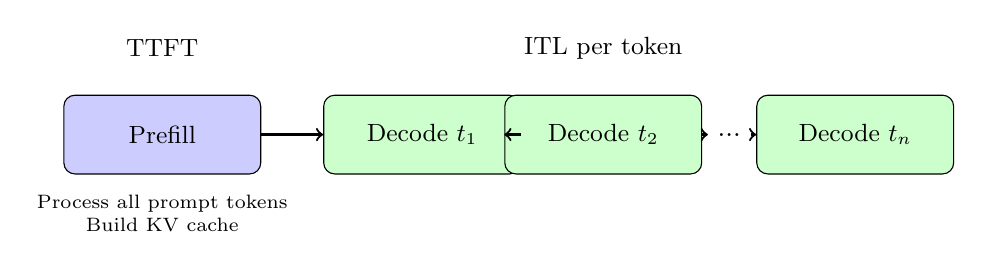
\begin{tikzpicture}[
    node distance=0.8cm,
    phase/.style={rectangle, draw, rounded corners, minimum width=2.5cm, minimum height=1cm, font=\small},
    prefill/.style={phase, fill=blue!20},
    decode/.style={phase, fill=green!20},
    arrow/.style={->, thick}
]
% Prefill
\node[prefill] (pf) {Prefill};
\node[below of=pf, yshift=-0.2cm, font=\scriptsize, align=center] (pf-desc) {Process all prompt tokens\\Build KV cache};

% Decode steps
\node[decode, right of=pf, xshift=2.5cm] (d1) {Decode $t_1$};
\node[decode, right of=d1, xshift=1.5cm] (d2) {Decode $t_2$};
\node[right of=d2, xshift=0.8cm] (dots) {...};
\node[decode, right of=dots, xshift=0.8cm] (dn) {Decode $t_n$};

% Arrows
\draw[arrow] (pf) -- (d1);
\draw[arrow] (d1) -- (d2);
\draw[arrow] (d2) -- (dots);
\draw[arrow] (dots) -- (dn);

% Labels
\node[above of=pf, yshift=0.3cm, font=\small] {TTFT};
\node[above of=d2, yshift=0.3cm, font=\small] {ITL per token};

\end{tikzpicture}
\caption{Inference lifecycle: prefill determines TTFT, decode determines generation speed.}
\label{fig:inference-lifecycle}
\end{figure}


\subsection{Stopping Conditions}
\label{subsec:stopping-conditions}

Generation continues until a stopping condition is met:

\begin{description}
\item[End-of-Sequence Token] The model outputs a special EOS token indicating it considers the response complete. This is the ``natural'' stopping point.

\item[Maximum Length] A hard limit on output tokens (e.g., \texttt{max\_tokens=500}). Essential for preventing runaway generation and controlling costs.

\item[Stop Sequences] Custom strings that halt generation when produced. Useful for structured outputs---stop at ``\textbackslash n\textbackslash n'' to get single paragraphs, or stop at ``\}'' when generating JSON.
\end{description}

\begin{lstlisting}[language=Python,caption={Stop sequence example}]
# Stop generation at specific patterns
response = generate(
    prompt="List three items:\n1.",
    stop=["\n4.", "\n\n"],  # Stop before 4th item or double newline
    max_tokens=100
)
\end{lstlisting}

% =============================================================================
\section{Why KV Cache Exists}
\label{sec:kv-cache}
% =============================================================================

The KV cache is the single most important optimization for transformer inference. Without it, generating long responses would be impractically slow. Understanding it explains why memory requirements grow with context length and why long-context models are challenging to deploy.

\subsection{The Naive Approach}
\label{subsec:naive-approach}

Consider what happens without caching. To generate token 100 in a sequence, the model must compute attention---and attention requires comparing the new token against all previous tokens.

In the naive approach:
\begin{itemize}
\item Generate token 1: Process 1 token through the model
\item Generate token 2: Process tokens 1--2 through the model (2 tokens)
\item Generate token 3: Process tokens 1--3 through the model (3 tokens)
\item ...
\item Generate token 100: Process tokens 1--100 through the model (100 tokens)
\end{itemize}

The total work to generate 100 tokens is $1 + 2 + 3 + ... + 100 = 5,050$ token-passes through the model. For 1,000 tokens, it's over 500,000. The complexity is $O(n^2)$ where $n$ is the sequence length.

This is absurdly wasteful. When generating token 100, we're recomputing attention for tokens 1--99 \emph{exactly as we did when generating token 99}. All that computation is redundant.

\subsection{The Key-Value Cache Optimization}
\label{subsec:kv-optimization}

The insight behind KV caching is simple: in autoregressive generation, the Keys and Values for previous tokens don't change. Token 50's Key is the same whether you're generating token 51 or token 500. So why recompute it?

The KV cache stores the Key and Value vectors for all previous tokens. During decode:
\begin{enumerate}
\item Compute K and V only for the new token
\item Append them to the KV cache
\item Compute attention using the new token's Query against \emph{all cached Keys}
\item Weight and sum the \emph{cached Values}
\end{enumerate}

Now the work per token is roughly constant---we just compute K, V, Q for one new token and do a lookup against the cache. Total work for 100 tokens drops from $O(n^2)$ to $O(n)$. That's the difference between impractical and real-time.

\begin{important}{The KV Cache Trade-off}
KV cache trades memory for compute. Instead of recalculating attention over all previous tokens, we store their key-value pairs and reuse them. This makes generation fast but consumes memory proportional to sequence length.
\end{important}

\subsection{How KV Cache Grows}
\label{subsec:kv-cache-growth}

The memory cost is the trade-off. For each token in the sequence, we must store its K and V vectors across all layers and all attention heads.

\begin{svgraybox}
\textbf{KV Cache Size Formula:}

\begin{equation}
\text{KV Cache (bytes)} = 2 \times L \times H \times D \times S \times B
\end{equation}

Where:
\begin{itemize}
\item $L$ = number of layers
\item $H$ = number of attention heads
\item $D$ = dimension per head
\item $S$ = sequence length
\item $B$ = bytes per value (2 for FP16)
\item Factor of 2 = one for Keys, one for Values
\end{itemize}
\end{svgraybox}

\calclink{/c/3/kv}{l=32&h=32&d=128&c=4096&b=2&n=1}{Try the interactive KV Cache calculator}

Let's calculate for a Llama 3.2 7B model at 4096 context length:
\begin{itemize}
\item Layers: 32
\item Heads: 32
\item Head dimension: 128
\item Sequence length: 4,096
\item Precision: FP16 (2 bytes)
\end{itemize}

\begin{equation}
\text{KV Cache} = 2 \times 32 \times 32 \times 128 \times 4096 \times 2 = 2.1 \text{ GB}
\end{equation}

That's 2 GB just for the KV cache---on top of the model weights themselves! At 128K context (increasingly common), the same model needs 68 GB for KV cache alone. This is why long-context models require substantial VRAM.

\begin{table}[htbp]
\centering
\caption{KV cache memory by model and context length (FP16).}
\label{tab:kv-cache-sizes}
\begin{tabular}{lrrrr}
\toprule
\textbf{Model} & \textbf{4K ctx} & \textbf{16K ctx} & \textbf{32K ctx} & \textbf{128K ctx} \\
\midrule
7B (32 layers)    & 2.1 GB   & 8.4 GB   & 16.8 GB  & 67 GB \\
13B (40 layers)   & 3.3 GB   & 13.1 GB  & 26.2 GB  & 105 GB \\
70B (80 layers)   & 10 GB    & 40 GB    & 80 GB    & 320 GB \\
\bottomrule
\end{tabular}
\end{table}

\subsection{The Memory vs Compute Trade-off}
\label{subsec:memory-compute-tradeoff}

KV cache creates a fundamental trade-off between memory and compute that shapes how we deploy models:

\begin{description}
\item[Without KV Cache] Each decode step recomputes attention from scratch. Low memory, high compute. Impractical for real-time generation.

\item[With KV Cache] Each decode step reads cached K/V. High memory, low compute. Fast generation but VRAM-limited.
\end{description}

This trade-off also explains why the two phases of inference have different characteristics:

\begin{itemize}
\item \textbf{Prefill} is compute-bound: We're processing many tokens in parallel, doing lots of matrix math. The GPU's tensor cores are busy.

\item \textbf{Decode} is memory-bound: We're reading the KV cache every step. The GPU is mostly waiting for memory access.
\end{itemize}

For systems engineers, this means different bottlenecks at different times. A prompt with 4,000 tokens followed by a 100-token response spends most of its latency in prefill. A short prompt with a long response spends most time in decode. Optimization strategies differ accordingly.

% Diagram: KV Cache Growth
\begin{figure}[htbp]
\centering
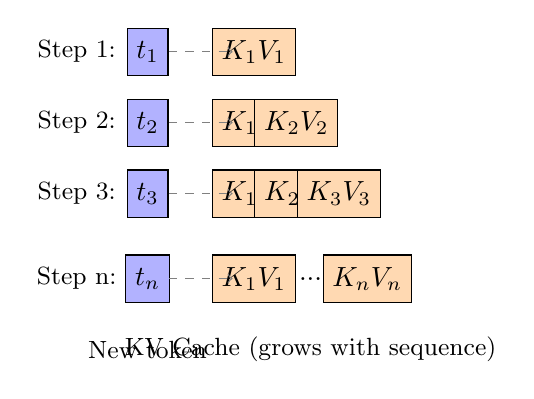
\begin{tikzpicture}[
    scale=0.9,
    cache/.style={rectangle, draw, fill=orange!30, minimum width=0.4cm},
    newtoken/.style={rectangle, draw, fill=blue!30, minimum width=0.4cm, minimum height=0.6cm}
]
% Step 1
\node at (-1, 2) {\small Step 1:};
\node[newtoken] at (0, 2) {$t_1$};
\node[cache, minimum height=0.6cm] at (1.5, 2) {$K_1V_1$};

% Step 2
\node at (-1, 1) {\small Step 2:};
\node[newtoken] at (0, 1) {$t_2$};
\node[cache, minimum height=0.6cm] at (1.5, 1) {$K_1V_1$};
\node[cache, minimum height=0.6cm] at (2.1, 1) {$K_2V_2$};

% Step 3
\node at (-1, 0) {\small Step 3:};
\node[newtoken] at (0, 0) {$t_3$};
\node[cache, minimum height=0.6cm] at (1.5, 0) {$K_1V_1$};
\node[cache, minimum height=0.6cm] at (2.1, 0) {$K_2V_2$};
\node[cache, minimum height=0.6cm] at (2.7, 0) {$K_3V_3$};

% Step n
\node at (-1, -1.2) {\small Step n:};
\node[newtoken] at (0, -1.2) {$t_n$};
\node[cache, minimum height=0.6cm] at (1.5, -1.2) {$K_1V_1$};
\node at (2.3, -1.2) {...};
\node[cache, minimum height=0.6cm] at (3.1, -1.2) {$K_nV_n$};

% Labels
\node at (0, -2.2) {\small New token};
\node at (2.3, -2.2) {\small KV Cache (grows with sequence)};

% Arrows showing cache read
\draw[->, gray, dashed] (0.3, 2) -- (1.2, 2);
\draw[->, gray, dashed] (0.3, 1) -- (1.2, 1);
\draw[->, gray, dashed] (0.3, 0) -- (1.2, 0);
\draw[->, gray, dashed] (0.3, -1.2) -- (1.2, -1.2);

\end{tikzpicture}
\caption{KV cache grows linearly: each new token adds its K/V to the cache and reads all previous entries.}
\label{fig:kv-cache-growth}
\end{figure}


% =============================================================================
\section{Key Metrics for Inference}
\label{sec:inference-metrics}
% =============================================================================

When evaluating inference performance, several metrics matter---and they can trade off against each other. Understanding what each metric measures helps you optimize for your specific use case.

\subsection{Time to First Token (TTFT)}
\label{subsec:ttft}

TTFT measures the delay from sending a request to receiving the first token of the response. This is the ``thinking time'' users perceive before the model starts responding.

TTFT is dominated by the prefill phase. A longer prompt means more tokens to process before generating can begin. For a chatbot, TTFT determines how long users wait before seeing any response.

\begin{svgraybox}
\textbf{Typical TTFT Values:}
\begin{itemize}
\item Short prompt (100 tokens), 7B model: 50--200ms
\item Medium prompt (1K tokens), 7B model: 200--500ms
\item Long prompt (10K tokens), 7B model: 1--3 seconds
\item Same prompts on 70B model: 3--10x longer
\end{itemize}
\end{svgraybox}

Applications like chat interfaces are sensitive to TTFT---users expect some acknowledgment quickly. Batch processing jobs care less; they're optimizing for total completion time.

\subsection{Inter-Token Latency (ITL)}
\label{subsec:itl}

ITL measures the time between consecutive output tokens. It determines how ``smooth'' streaming feels. Also called Time Between Tokens (TBT) or decode latency.

ITL is determined by the decode phase---one forward pass per token. Since decode is memory-bound, ITL depends heavily on memory bandwidth. Faster VRAM means lower ITL.

For a smooth streaming experience, ITL should be under 50ms. At 50ms per token, you're generating 20 tokens/second, which is comfortable reading speed. Above 100ms, users perceive choppiness.

\subsection{Tokens per Second}
\label{subsec:tokens-per-second}

Tokens per second is the inverse of ITL, measuring generation speed. It's the most commonly cited performance metric.

\begin{svgraybox}
\textbf{Typical Generation Speeds:}
\begin{itemize}
\item CPU inference (7B Q4): 5--15 tok/s
\item RTX 4060 (7B Q4): 40--60 tok/s
\item RTX 4090 (7B Q4): 80--120 tok/s
\item A100 80GB (7B FP16): 150--200 tok/s
\item H100 (7B FP16): 200--400 tok/s
\end{itemize}
\end{svgraybox}

For context: average reading speed is about 250 words per minute, roughly 5--6 tokens per second. Even modest GPU inference outpaces human reading. The real question is whether the speed is sufficient for your application's latency requirements.

\subsection{Throughput}
\label{subsec:throughput}

Throughput measures how many requests (or total tokens) your system can handle per unit time. It's a system-level metric, distinct from single-request speed.

The key insight: throughput and latency trade off. Batching multiple requests together increases throughput (more efficient GPU utilization) but increases latency for individual requests (each waits for the batch).

Production systems use \emph{continuous batching}---dynamically adding new requests to an in-progress batch. This achieves high throughput while keeping latency bounded. Chapter~\ref{ch:inference-engines} covers vLLM's implementation in detail.

% Diagram: Metrics Visualization
\begin{figure}[htbp]
\centering
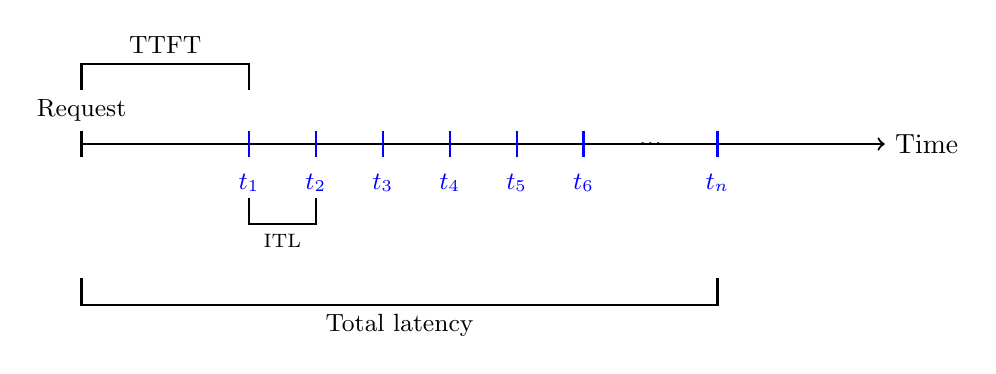
\begin{tikzpicture}[scale=0.85]
% Timeline
\draw[thick, ->] (0, 0) -- (12, 0) node[right] {Time};

% Request marker
\draw[thick] (0, -0.2) -- (0, 0.2);
\node[above] at (0, 0.2) {\small Request};

% TTFT bracket
\draw[thick] (0, 0.8) -- (0, 1.2) -- (2.5, 1.2) -- (2.5, 0.8);
\node[above] at (1.25, 1.2) {\small TTFT};

% First token
\draw[thick, blue] (2.5, -0.2) -- (2.5, 0.2);
\node[below, blue] at (2.5, -0.3) {\small $t_1$};

% ITL brackets
\draw[thick] (2.5, -0.8) -- (2.5, -1.2) -- (3.5, -1.2) -- (3.5, -0.8);
\node[below] at (3, -1.2) {\scriptsize ITL};

% Subsequent tokens
\foreach \x/\n in {3.5/2, 4.5/3, 5.5/4, 6.5/5, 7.5/6} {
    \draw[thick, blue] (\x, -0.2) -- (\x, 0.2);
    \node[below, blue] at (\x, -0.3) {\small $t_{\n}$};
}

\node at (8.5, 0) {...};

% Final token
\draw[thick, blue] (9.5, -0.2) -- (9.5, 0.2);
\node[below, blue] at (9.5, -0.3) {\small $t_n$};

% Total time bracket
\draw[thick] (0, -2) -- (0, -2.4) -- (9.5, -2.4) -- (9.5, -2);
\node[below] at (4.75, -2.4) {\small Total latency};

\end{tikzpicture}
\caption{Inference timing: TTFT is time to first token, ITL is time between subsequent tokens.}
\label{fig:inference-timing}
\end{figure}


\begin{table}[htbp]
\centering
\caption{Inference metrics summary.}
\label{tab:inference-metrics}
\begin{tabular}{llll}
\toprule
\textbf{Metric} & \textbf{Measures} & \textbf{Target} & \textbf{Affected By} \\
\midrule
TTFT & Responsiveness & <1s & Prompt length, model size \\
ITL & Streaming smoothness & <50ms & Model size, memory bandwidth \\
Tokens/sec & Generation speed & >30 & GPU power, quantization \\
Throughput & System capacity & Varies & Batching, hardware \\
\bottomrule
\end{tabular}
\end{table}

\subsection{What Affects Each Metric}
\label{subsec:metric-factors}

Different hardware and configuration choices affect metrics differently:

\begin{description}
\item[TTFT] Primarily affected by prompt length and model size. Faster GPU compute helps (prefill is compute-bound). Quantization has modest impact since compute is the bottleneck.

\item[ITL] Primarily affected by memory bandwidth. Faster VRAM helps. Quantization helps significantly---smaller values mean less data to read from memory.

\item[Tokens/sec] Inverse of ITL. Same factors apply.

\item[Throughput] Affected by everything: GPU compute, memory, batch size, model size. Continuous batching is the key optimization. More VRAM allows larger batches.
\end{description}

\begin{important}{The Optimization Target Depends on Use Case}
\begin{itemize}
\item \textbf{Interactive chat}: Optimize TTFT and ITL for responsiveness
\item \textbf{Batch processing}: Optimize throughput; latency less important
\item \textbf{Real-time API}: Balance all metrics; set SLO targets for each
\item \textbf{Code completion}: TTFT is critical (users wait for suggestions)
\end{itemize}
\end{important}

% =============================================================================
\section{Other Model Architectures}
\label{sec:other-architectures}
% =============================================================================

While decoder-only transformers dominate LLM inference, several other architectures are worth understanding. They have different memory and compute characteristics that affect deployment decisions.

\subsection{Mixture of Experts (MoE)}
\label{subsec:moe}

MoE models replace the single feed-forward network with multiple ``expert'' FFNs. A learned router decides which experts process each token. Not all parameters are active for every token.

% Diagram: MoE Architecture
\begin{figure}[htbp]
\centering
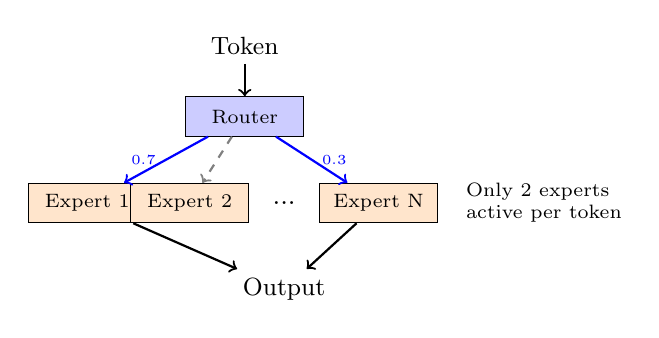
\begin{tikzpicture}[
    node distance=0.6cm,
    block/.style={rectangle, draw, minimum width=1.5cm, minimum height=0.5cm, font=\scriptsize},
    expert/.style={block, fill=orange!20},
    router/.style={block, fill=blue!20},
    arrow/.style={->, thick}
]
% Input
\node (input) {\small Token};

% Router
\node[router, below of=input, yshift=-0.3cm] (router) {Router};

% Experts
\node[expert, below of=router, xshift=-2cm, yshift=-0.5cm] (e1) {Expert 1};
\node[expert, below of=router, xshift=-0.7cm, yshift=-0.5cm] (e2) {Expert 2};
\node[below of=router, xshift=0.5cm, yshift=-0.5cm] (dots) {...};
\node[expert, below of=router, xshift=1.7cm, yshift=-0.5cm] (en) {Expert N};

% Output
\node[below of=dots, yshift=-0.5cm] (output) {\small Output};

% Arrows
\draw[arrow] (input) -- (router);
\draw[arrow, blue, thick] (router) -- (e1) node[midway, left, font=\tiny] {0.7};
\draw[arrow, gray, dashed] (router) -- (e2);
\draw[arrow, blue, thick] (router) -- (en) node[midway, right, font=\tiny] {0.3};
\draw[arrow] (e1) -- (output);
\draw[arrow] (en) -- (output);

% Annotation
\node[right of=en, xshift=1.5cm, align=left, font=\scriptsize] {Only 2 experts\\active per token};

\end{tikzpicture}
\caption{MoE: router selects which experts process each token. Most experts stay idle.}
\label{fig:moe-architecture}
\end{figure}


\begin{backgroundinformation}{MoE Example: Mixtral 8x7B}
Mixtral 8x7B has 8 experts, each roughly 7B parameters. But only 2 experts are active per token. Total parameters: $\sim$47B. Active parameters: $\sim$13B.

\textbf{Implications:}
\begin{itemize}
\item \textbf{Inference speed}: Similar to a 13B dense model (only active params compute)
\item \textbf{Quality}: Closer to a 47B dense model (more total capacity)
\item \textbf{Memory}: Still need $\sim$47B worth of VRAM (all experts loaded)
\end{itemize}
\end{backgroundinformation}

MoE models are attractive when you want larger-model quality at smaller-model speed, \emph{if} you have the memory. They don't save VRAM---they trade speed for quality at fixed memory.

\subsection{Diffusion Models}
\label{subsec:diffusion}

Diffusion models power image generation (Stable Diffusion, DALL-E, Midjourney) and increasingly video. They work fundamentally differently from LLMs:

\begin{itemize}
\item \textbf{No autoregression}: Generate the entire output simultaneously, not token-by-token
\item \textbf{Iterative denoising}: Start with noise, gradually refine over many steps (20--50 typically)
\item \textbf{No KV cache}: No sequential dependency between ``tokens''
\item \textbf{U-Net architecture}: Often not transformers at all (though DiT uses transformers)
\end{itemize}

Memory characteristics differ: no KV cache growth, but need to store multiple versions of the image during denoising. Inference time scales with step count, not output size.

This book focuses on LLMs, but many inference concepts apply: batching, quantization, and GPU optimization.

\subsection{Multimodal Models}
\label{subsec:multimodal}

Multimodal models handle multiple input types---typically text and images. Examples include LLaVA, GPT-4V, and Gemini.

Architecture typically combines:
\begin{itemize}
\item \textbf{Vision encoder}: Processes images into embeddings (often a pretrained CLIP or ViT)
\item \textbf{Projection layer}: Converts image embeddings to match LLM's dimension
\item \textbf{LLM backbone}: Standard decoder-only transformer for text generation
\end{itemize}

Memory implications:
\begin{itemize}
\item Additional VRAM for vision encoder ($\sim$300M--2B parameters)
\item Image embeddings added to context (one image $\approx$ 256--576 tokens worth)
\item KV cache includes image token representations
\end{itemize}

Deploying multimodal models requires planning for both the vision and language components.

\subsection{State Space Models}
\label{subsec:ssm}

State Space Models (SSMs) like Mamba offer an alternative to attention with different scaling properties:

\begin{itemize}
\item \textbf{Linear complexity}: $O(n)$ instead of attention's $O(n^2)$ for sequence length
\item \textbf{No KV cache}: State is fixed-size regardless of context length
\item \textbf{Recurrent-like}: Processes tokens sequentially but with efficient parallel training
\end{itemize}

\begin{svgraybox}
\textbf{SSM Trade-offs:}
\begin{itemize}
\item \textbf{Pro}: Constant memory per token, no KV cache explosion
\item \textbf{Pro}: Potentially faster for very long sequences
\item \textbf{Con}: Less mature ecosystem and tooling
\item \textbf{Con}: Quality may lag behind transformers on some tasks
\item \textbf{Con}: Hybrid models (Mamba + attention) gaining popularity
\end{itemize}
\end{svgraybox}

SSMs are an active research area. As of early 2025, transformers remain dominant, but SSMs are worth watching for long-context applications.

% =============================================================================
\section{Summary}
\label{sec:ch02-summary}
% =============================================================================

This chapter provided the conceptual foundation for understanding LLM inference. We traced the evolution from sequential RNNs to parallel transformers, explored the attention mechanism that allows tokens to communicate, and walked through the inference lifecycle from prompt tokenization through autoregressive generation.

The key insight is the KV cache: by caching attention key-value pairs, we trade memory for dramatic compute savings. This trade-off is central to everything that follows---VRAM requirements, context length limits, and optimization strategies all flow from this fundamental architecture.

With this mental model in place, Chapter~\ref{ch:hardware-fundamentals} will quantify these concepts: exactly how much memory does a 7B model need? How does quantization reduce that? When does CPU inference make sense? The formulas will make more sense now that you understand what they're measuring.

\begin{important}{Key Takeaways}
\begin{itemize}
\item Transformers process all tokens in parallel (prefill) then generate one at a time (decode)
\item The ``billions'' in 7B are learnable parameters---weights stored as floating point numbers
\item KV cache trades memory for compute, enabling fast autoregressive generation
\item Memory grows linearly with sequence length due to KV cache
\item Key metrics: TTFT (responsiveness), ITL (smoothness), tokens/sec (speed), throughput (capacity)
\item MoE models have many parameters but only activate a subset per token
\end{itemize}
\end{important}

% =============================================================================
\section*{Problems}
\addcontentsline{toc}{section}{Problems}
% =============================================================================

\begin{prob}
\label{prob:ch02-kv-cache}
\textbf{KV Cache Calculation}\\
A model has 32 layers, 32 attention heads, 128 dimensions per head, and uses FP16 precision. Calculate the KV cache size for a 4096-token context. Then calculate for an 8192-token context.
\end{prob}

\begin{prob}
\label{prob:ch02-ttft-vs-itl}
\textbf{TTFT vs ITL}\\
Explain why a model might have excellent TTFT but poor ITL, or vice versa. What hardware characteristics would cause each scenario?
\end{prob}

\begin{prob}
\label{prob:ch02-moe-memory}
\textbf{MoE Memory Requirements}\\
Mixtral 8x7B has 8 experts with 7B parameters each, but only 2 experts are active per token. Explain why you still need memory for all 47B parameters, not just 14B.
\end{prob}

%%%%%%%%%%%%%%%%%%%%%%%% references02.tex %%%%%%%%%%%%%%%%%%%%%%%%%%%%%%
% References for Chapter 2
%%%%%%%%%%%%%%%%%%%%%%%% Springer-Verlag %%%%%%%%%%%%%%%%%%%%%%%%%%

\begin{thebibliography}{99.}

\bibitem{nvidia2024h100} NVIDIA: H100 Tensor Core GPU Datasheet. \url{https://www.nvidia.com/en-us/data-center/h100/} (2024)

\bibitem{nvidia2024a100} NVIDIA: A100 Tensor Core GPU Datasheet. \url{https://www.nvidia.com/en-us/data-center/a100/} (2024)

\bibitem{amd2024mi300} AMD: Instinct MI300X Accelerator. \url{https://www.amd.com/en/products/accelerators/instinct/mi300/mi300x.html} (2024)

\bibitem{apple2024m4} Apple: M4 Chip Architecture. \url{https://www.apple.com/newsroom/2024/05/apple-introduces-m4-chip/} (2024)

\bibitem{runpod2025pricing} RunPod: GPU Cloud Pricing. \url{https://www.runpod.io/gpu-instance/pricing} (accessed December 2025)

\bibitem{vastai2025} Vast.ai: GPU Marketplace. \url{https://vast.ai/} (accessed December 2025)

\bibitem{lambdalabs2025} Lambda Labs: GPU Cloud. \url{https://lambdalabs.com/service/gpu-cloud} (accessed December 2025)

\end{thebibliography}

